\documentclass{article}
\usepackage[utf8]{inputenc}
\usepackage[italian]{babel}
\usepackage{graphicx}
\usepackage{xcolor}
\usepackage[a4paper,top=15mm, bottom=15mm, left=15mm, right=15mm]{geometry}
\begin{document}
		\author{Alessandro Fuser}
		\title{Vivi Internet al meglio}
		\maketitle
		\begin{figure}[h!]
			\centering
			
\includegraphics[scale=0.8]{logo.png}
		\end{figure}
		
		\pagebreak
		
		\tableofcontents
		
		\pagebreak
		
		\section{L'ombra digitale}
		In questa sezione, imparerai a capire cos'è l'ombra digitale, a valutare il peso delle nostrea azioni nel mondo del Web nel tempo e a tutelare la privacy delle persone.
		\subsection{L'ombra digitale}
		Alcuni “errori” commessi su Internet in età giovanissima possono “estendersi” come un’ombra e comportare danni alla reputazione permanenti. Foto, audio, video, testi, post di blog e messaggi scritti o registrati sui propri account e profili, ma anche su quelli di amici o conoscenti, rimangono in rete come impronte.\\
		\textbf{Curare la propria identità e reputazione digitale non solo per l'oggi, ma anche per il proprio futuro}.\\
		Addirittura, oggi, anche le aziende si informano e si interessano ai profili social dei candidati, per ricostruirne, insieme ad altri elementi, il profilo socioculturale, relazionale e valoriale e valutarne l’inserimento in azienda.\\
		\textbf{L’ombra digitale non è altro che la nostra impronta elettronica, alimentata dal modo con cui ci rapportiamo con la tecnologia.} Quando pubblichiamo una foto, ci registriamo in un luogo, inviamo un messaggio vocale, lasciamo un commento, iniziamo a seguire una pagina o un gruppo, etc. non facciamo altro che alimentare la nostra ombra digitale, lasciamo tracce di noi. La nostra ombra digitale può dire molte cose di noi e afferisce alla nostra privacy. \\
		\begin{figure}[h!]
			\centering
			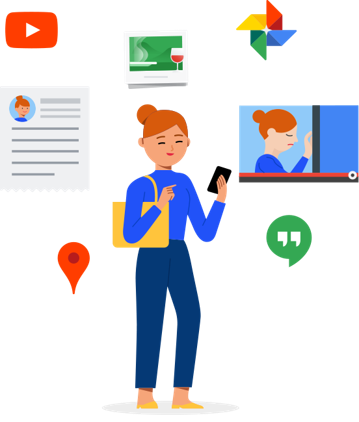
\includegraphics[scale=0.5]{Image1.png}
		\end{figure}
		\newline
		Sul web, condividiamo informazioni in modo volontario, ma non sempre consapevole delle possibili conseguenze. Sui blog o social network (Facebook, Snapchat, YouTube, etc) gli utenti tracciano un proprio profilo, inseriscono una descrizione di se stessi, costruiscono liste di amici o di cose che amano, pubblicano foto o video, stabiliscono relazioni sociali ed affettive, condividono cose, collegano tra loro profili e piattaforme social diverse, etc. È importare riconoscere e valutare quali informazioni e quali azioni in rete hanno un impatto maggiore sulla creazione della nostra ombra e identità digitale.\\
		\subsubsection{Caso di studio}
		\label{sec:Caso1}
		Lorenzo, che è prossimo alla maturità, con alcuni amici di classe gira di nascosto un video nei bagni della scuola. Registra conversazioni, atteggiamenti e scene che nessuno può immaginare finiranno in rete. Lorenzo e i suoi amici postano il video su una chat di gruppo della scuola, ma qualcuno, dopo qualche giorno, condivide il video all’esterno della chat sino ad arrivare al preside, che lo mostra anche ai genitori.
		\\\vspace{5mm}\\
		\textbf{Cosa si potrebbe pensare di Lorenzo e dei suoi amici, non conoscendoli e guardando quel video?}
		\begin{itemize}
			\item Che sono ragazzi superficiali;
			\item Che sono ragazzi divertenti e simpatici
			\item Che sono ragazzi poco attenti alla reputazione dei loro amici
			\item Che sono ragazzi abili con le nuove tecnologie
		\end{itemize}
	\subsubsection{Caso di studio}
	\label{sec:Caso2}
	Luca è un writer e nel tempo libero realizza graffiti su commissione, per privati o in spazi pubblici adibiti dal Comune a tale scopo. Sui social e sul suo canale YouTube pubblica foto e video che mostrano dettagli dei suoi lavori o lo ritraggono all'opera, appeso ad un cavo, spesso di notte, da solo, senza alcun riferimento sui luoghi o sui committenti delle sue opere. Molti amici di Luca, scherzosamente, si rivolgono a lui chiamandolo "writer clandestino" e postano commenti del tipo "Quale altro muro avrai imbrattato oggi?"
	\\\vspace{5mm}\\
	\textbf{Se un domani Luca dovesse partecipare ad un colloquio per l’alternanza scuola lavoro e il responsabile delle risorse umane si imbattesse nei suoi profili social, che idea potrebbe farsi leggendo i commenti sulla sua pagina o sul suo canale video? Quale ombra digitale potrebbe emergere dal suo profilo?}
	\begin{itemize}
		\item Quella di un ragazzo con una passione sana per l’arte, socievole e con uno spiccato senso civico;
		\item Quella di un writer non autorizzato e privo di senso civico;
		\item Quella di un ragazzo poco affidabile e senza alcun controllo da parte della famiglia: un giovane di quell’età che passa le nottate fuori di casa!
	\end{itemize}
	\subsection{Il peso delle nostre azioni nel tempo}
	\begin{figure}[h!]
		\centering
		
\includegraphics[scale=0.2]{Image2.png}
	\end{figure}
	Vi sono informazioni piuttosto comuni che possono essere condivise su piattaforme social, siti web, gruppi, app mobile, etc. che possono contenere dettagli importanti sulla nostra vita e le nostre abitudini. Bisognerebbe sempre valutare il grado di rischio e di impatto sulla privacy che ogni elemento condiviso potrebbe avere e considerare anche l’impatto che queste informazioni potrebbero avere sulla privacy di altri individui, oltre che su quella di chi le sta condividendo. 
	Facciamo dei facili ma evidenti esempi:
	\begin{enumerate}
		\item Le informazioni sui luoghi e i locali che frequentiamo, e che con un solo click condividiamo, grazie a servizi di geolocalizzazione possono rappresentare delle impronte e delle informazioni sensibili, a disposizione potenzialmente di chiunque
		\item La registrazione dei ragazzi presso palestre, locali, scuole, può fornire informazioni molto precise sui loro spostamenti e sulle loro abitudini
		\item Immagini e informazioni della propria abitazione possono fornire a malintenzionati materiale utile per possibili azioni fraudolente e dannose per noi e il nostro nucleo familiare
		\item Il tag di un amico in una foto geolocalizzata può fornire informazioni, anche sul suo conto, che magari personalmente avrebbe evitato di condividere pubblicamente
	\end{enumerate}
	\subsubsection{Caso di studio}
	\label{sec:Caso3}
	Francesco, che è un tipo molto scherzoso, condivide una foto sulla bacheca della sua amica Carla che mostra un “6 in condotta” ottenuto al primo quadrimestre, ma in realtà si tratta di uno scherzo. Quel 6 non è del ragazzo, e quella condivisa è un’immagine trovata sul web. Lo fa per colpire Carla e innescare stupore e clamore sui social. A distanza di alcuni mesi Francesco, che nel tempo libero si occupa di consegne a domicilio, risponde ad un annuncio di lavoro e viene chiamato per un colloquio. Fra gli esercizi commerciali che vogliono usufruire del servizio c’è il titolare di una paninoteca, amico di Carla, che riconosce Francesco e ricorda la superficialità con cui il ragazzo aveva reagito al 6 in condotta.
	\\\vspace{5mm}\\
	\textbf{Cosa avresti potuto consigliare a Francesco per evitare questa situazione?}
	\begin{itemize}
		\item Di inviare la foto in un messaggio privato
		\item Di impostare "Solo amici" sul suo profilo
		\item Di impostare "Tutti" sul profilo della sua amica
		\item Di esplicitare, dopo qualche giorno, che si trattava di uno scherzo e/o eliminare l'immagine
	\end{itemize}
\subsubsection{Caso di studio}
\label{sec:Caso4}
Claudio partecipa ad una festa di 18 anni. La serata si accende, tutti si lasciano un po’ andare e iniziano a scambiarsi battute fuori dagli schemi; anche Claudio si lascia trascinare pronunciando cose che mai avrebbe detto fuori da un contesto goliardico. Il video, a distanza di anni, finisce in una playlist di video pubblica e diventa virale. Claudio è riconoscibilissimo. In rete si scatena un passaparola su Claudio che lo pone in grande imbarazzo.
\\\vspace{5mm}\\
\textbf{Cosa avresti potuto consigliare a Claudio per evitarlo?}
\begin{itemize}
	\item Di controllare le impostazioni e le notifiche sui tag
	\item Di evitare di farsi riprendere
	\item Di impostare il video come "non visibile sul suo profilo"
	\item Di segnalare il video
\end{itemize}
\subsection{La tutela della privacy}
\textbf{La tutela della propria privacy è importante, la tutela della privacy degli altri è “sacra”.} Ogni volta che condividiamo un contenuto, un’immagine, un video, un messaggio vocale, etc. dovremmo chiederci se quel contenuto riguarda solo noi o se sta, anche indirettamente, coinvolgendo ed esponendo qualcun altro. Vi sono informazioni che in alcuni casi sentiamo l’esigenza di condividere, ma spesso si tratta di contenuti che potrebbero rappresentare una confidenza intima, delle informazioni delicate, che varrebbe la pena tenere tra noi e poche altre persone.
\\\vspace{5mm}\\
Facciamo un esempio: un conoscente molto più grande di Luna che sa della sua passione per il ciclismo, la invita in una chat di gruppo su smartphone creata per condividere informazioni e organizzare gite in mountain bike. Il suo nome inizia a circolare perché ha fatto un'ottima figura alla prima uscita di gruppo. Alcuni dei partecipanti alla chat le chiedono l’amicizia sui social, sebbene lei non li conosca ancora bene. Uno di loro inizia a scriverle in una chat privata parallela e la invita a visitare il suo garage pieno di pezzi di ricambio. Luna accetta l’invito e in quella occasione le regala una coppia di pedali molto rari. Nei giorni successivi la invita nuovamente e per obbligo e gratitudine Luna ritorna a trovarlo. In quella occasione l'uomo insiste per regalarle un altro pezzo di ricambio. Luna è imbarazzata, ma non riesce a rifiutare. Gli inviti e i messaggi si fanno sempre più insistenti, Luna inizia a non rispondere più ai messaggi, trova delle scuse e gli dice che ha molto da fare con la scuola. Lui inizia a chiamarla direttamente sul cellulare. Qualche settimana dopo, uscendo dalla palestra, lo trova inaspettatamente fuori ad attenderla: le fa una scenata, accusandola di ingratitudine e le dà l’impressione di essere fuori controllo. Luna si spaventa molto!
\\\vspace{5mm}\\
\textbf{Come avrebbe potuto evitare questa situazione imbarazzante?}\\
La palestra è tra i luoghi in cui ci si registra in maniera ricorrente sui Social e il numero di cellulare è in chiaro nelle chat di gruppo come WhatsApp. Per questa ragione quando si accetta che qualcuno ci inserisca in un gruppo di chat o si accetta l’amicizia sui social di persone che conosciamo benissimo, \textit{bisogna chiedersi quali informazioni personali saranno immediatamente a loro disposizione}.\\
È bello fidarsi dei propri amici, ma è sempre meglio chiedersi se quello che condividiamo con loro sul web o sulle chat mobile, corre il rischio di essere volontariamente promulgato o fraudolentemente sottratto da perfetti sconosciuti.\\
\textcolor{red}{Attenzione!} Ogni volta che condividete codici di sblocco o password su social e chat di gruppo, ricordate che vi state esponendo a due tipologie di rischio, una goliardata più o mena faceta da parte del vostro entourage di amici, ma anche la diffusione involontaria delle vostre password a estranei malintenzionati
\subsubsection{Caso di studio}
\label{sec:Caso5}
Simona organizza una festa a casa sua per il suo compleanno. Utilizza una chat di gruppo per condividere con gli invitati orario e indirizzo. I suoi amici iniziano ad arrivare, ma per aprire il cancello ed entrare c’è bisogno di digitare un codice sul citofono, dopo il quarto squillo di campanello, Simona decide di scrivere il codice sulla chat di gruppo per godersi la festa e non passare tutta la serata al citofono. La settimana dopo la casa dei suoi genitori viene svaligiata, senza alcun segno di effrazione. Dopo qualche giorno Simona scopre che ad una sua amica hanno rubato la borsa sull’autobus e il suo dispositivo non era protetto da password.
\\\vspace{5mm}\\
\textbf{Cosa avrebbe potuto evitare questa situazione a Simona e i suoi genitori?}
\begin{itemize}
	\item Non condividere mai e per nessuna ragione una password (per intero) in una chat
	\item Cancellare il gruppo dopo la festa
	\item Cancellare il messaggio dopo la festa
	\item Scrivere la password in più messaggi differenti
\end{itemize}
\subsection{Rischi per la privacy}
Tra le informazioni sensibili che ci riguardano ve ne sono alcune che possono causare problemi che vanno oltre la privacy e arrecare perdite finanziarie. Oltre alle pratiche di phishing vere e proprie, che spesso simulano richieste di istituti bancari o affini, ci sono anche delle cattive abitudini di condivisione che possono metterci a rischio.
\subsubsection{Caso di studio}
\label{sec:Caso6}
Il padre di Ben gli ha promesso che appena gli sarà possibile metterà a disposizione la sua carta di credito per prenotare il viaggio a Londra che farà con i suoi amici. Si è offerto di anticipare le spese per tutti e cinque i suoi compagni. Nella chat del viaggio alcuni dei suoi amici hanno fretta e iniziano a fargli pressione. Iniziano a circolare battute: “cocco di papà”, “pappa molla”, etc. A Ben non piace essere deriso e non vuole che a causa sua qualcosa possa andare storto. Una sera, mentre suo padre dorme, prende la sua carta di credito e condivide tutti i dati in chat affinché gli altri si diano da fare per prenotare il Volo+Hotel desiderato. Uno dei suoi compagni di classe, che inizialmente doveva partire con loro, ma che per una incomprensione non parteciperà più al viaggio, è ancora parte della chat e per fargli uno scherzo, con i dati della carta prenota uno spettacolo per adulti in un locale di Londra, ad un costo piuttosto elevato. Il padre di Ben l’indomani mattina, vede le notifiche delle transazioni sul cellulare e si accorge che, oltre al Volo+Hotel, c’è anche un addebito per uno spettacolo per adulti a una cifra esorbitante, non rimborsabile. 
\\\vspace{5mm}\\
\textbf{Cosa avrebbe dovuto fare per evitarli?}
\begin{itemize}
	\item Aspettare il padre		
	\item Chiedere al padre di condividere i dati della carta di credito a pezzi e su piattaforme e canali differenti		
	\item Fotografare la carta e inviare una foto invece dei dati		
	\item Condividere i dati della carta via mail		
	\item Condividerli tutti contemporaneamente su una chat
\end{itemize}
\subsection{Codici Personali}
È sempre sconsigliato utilizzare chat, app, email, per condividere codici personali, password, estremi di una carta di credito o gli accessi al proprio conto corrente. Le regole fondamentali per la condivisione dei propri codici personali sono:
\begin{enumerate}
	\item La persona deve essere di nostra conoscenza ed affidabile
	\item Evitare di condividere i dati e le informazioni con più persone contemporaneamente
	\item Non utilizzare le piattaforme web (o solo piattaforme web)
	\item Se strettamente necessario meglio suddividere la comunicazione dei dati su piattaforme e canali differenti
	\item Evitare nelle comunicazioni di esplicitare che si tratta di password o numeri di carta di credito
	\item Evitare di eseguire queste operazioni su un wifi pubblico
\end{enumerate}\begin{figure}[h!]
\centering
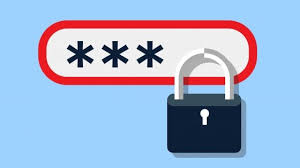
\includegraphics[scale=0.5]{Image3.jpg}
\end{figure}
Di seguito fornisco degli esempi chiarificativi sulla violazione della privacy altrui:
\begin{enumerate}
	\item Tua sorella minore si è bruciata con dell’acqua bollente e l’ustione le ha provocato brutte ferite sul volto e sulle mani. Non vuole che altre persone lo sappiano o la vedano così. Un tuo caro amico viene a trovarti e scatta delle foto e gira dei video a sua insaputa e li condivide su Instagram e YouTube. Iniziano ad arrivare commenti di compassione e altri di disgusto
	\item Scrivi un pensiero sul tuo diario che riguarda un/a ragazzo/a che ti piace molto. Qualcuno scatta una foto a quello che hai scritto e la condivide sui social.
	\item Qualcuno scrive "Buone vacanze" sul profilo social di un amico.	La persona che sta per partire lo aveva annunciato pubblicamente?
\end{enumerate}
\begin{center}
	\begin{huge}
		\textbf{CONDIVIDI USANDO IL BUON SENSO!}
	\end{huge}
\end{center}
%\begin{figure}[h!]
%	\centering
%	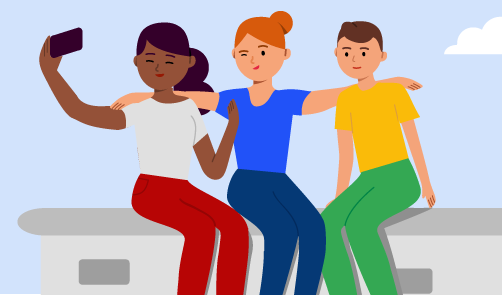
\includegraphics[scale=1]{Image4.png}
%\end{figure}

\pagebreak

\section{Impara a distinguere il vero dal falso}
In questa sezione andremo a capire cos'è il phishing, a come riconoscere i tentativi di frode ed evitare gli sconosciuti in rete.
\subsection{Il Phishing}
\begin{figure}[h!]
	\centering
	
\includegraphics[scale=0.7]{VeroFalso.jpg}
\end{figure}
\textbf{Il phishing è un tipo di truffa che consiste nel procurarsi in maniera fraudolenta dati riservati delle proprie vittime.} Può consistere nel sottrarre dati sensibili agli utenti per rivenderli a società pubblicitarie, rubare denaro tramite il furto di credenziali bancarie o semplicemente infettare i dispositivi con virus in grado di appropriarsi dell'elenco dei contatti per inviare email di phishing anche a loro. È un tentativo fraudolento che spesso utilizza Brand noti all’utente, verso i quali si nutre fiducia, per cercare di ottenere dati personali.\\
Accade che messaggi, spessissimo inviati via email, apparentemente da entità note e reali come banche, siti di prenotazione, etc. sollecitano il destinatario a fare clic su un link per verificare account personali al fine di rafforzare la sicurezza o in cambio di benefici o servizi gratuiti. Queste pratiche consentono ai malintenzionati di ottenere l'accesso da remoto ai dispositivi dei malcapitati o di impossessarsi di informazioni sensibili, come nome utente, password o, nei casi peggiori, dei dati della carta di credito o di altre forme di pagamento online.\\
A volte il phishing utilizza strumenti apparentemente innocui come email o post in cui viene chiesto di far girare un dato messaggio a tutti i propri contatti, le famose catene di Sant’Antonio. Sistemi utilizzati per raccogliere massivamente indirizzi a cui inviare pubblicità di vario genere (spam), o addirittura veicolare virus tramite link predisposti ad hoc, o nascondere vere e proprie truffe. \textbf{Per questo motivo è importantissimo prestare sempre la massima attenzione al controllo dei propri account sul web e attivare nella casella di posta i filtri antispam.}\\
\textcolor{red}{Attenzione!} Bisogna sempre verificare con attenzione un messaggio che offre in modalità completamente gratuita qualcosa che ha un valore economico oggettivo.\\
Molti tentativi di frode online possono avvenire anche tramite piattaforme social. Ad esempio sulle pagine di personaggi pubblici o celebrità può accadere che, tra i commenti ai post, un utente inserisca un link fraudolento per offrire ingressi gratuiti, biglietti di concerti, etc.\\
\textcolor{blue}{Banche, enti pubblici, aziende e grandi catene di vendita non richiedono informazioni personali attraverso email, sms, social media o chat.}
\subsection{Riconoscere i tentativi di frode}
Una buona prassi per riconoscere i tentativi di frode è di fare attenzione a queste semplici situazioni:
\begin{enumerate}
	\item Normalmente le offerte gratuite non sono davvero tali
	\item Alcuni siti ti chiedono informazioni personali apparentemente banali ma da cui è possibile desumere informazioni sensibili. Per esempio, i "test della personalità" potrebbero raccogliere dati per riuscire a indovinare la tua password o sottrarti altre informazioni private. La maggior parte delle imprese reali, viceversa, non richiede informazioni personali via email
	\item Le email e i post in cui ti viene chiesto di far girare il messaggio a tutti i tuoi contatti possono mettere a rischio te e altre persone. Non farli girare a meno che tu non conosca la fonte e sappia con certezza che il messaggio è sicuro
	\item In fondo alla maggior parte dei documenti puoi trovare delle note scritte con caratteri più piccoli. Questa parte di testo spesso contiene informazioni importanti scritte in piccolo di modo che tu non le legga. Per esempio, potrebbe esserci un titolo in cui ti viene annunciato che hai vinto un telefono in omaggio, ma in piccolo c'è scritto che per averlo devi pagare 200 euro al mese
\end{enumerate}
\subsubsection{Caso di studio}
\label{sec:Caso7}
Una della vostra classe riceve questo messaggio sul cellulare in merito ad una notissima marca di abbigliamento "Buono di 150 euro. Ricevi un coupon di Nome Marca del valore di 150 euro clicca su nomemarca.coupongratis.com. Io l'ho appena preso, sbrigati non perdere tempo! :D" Lo gira a tutta la classe e anche a te, pensando di fare una cosa gradita.
\\\vspace{5mm}\\
\textbf{Cosa le avresti consigliato di fare?}
\begin{itemize}
	\item Ignorare il messaggio e non cliccare		
	\item Cliccare per capire di cosa si tratta		
	\item Inviarlo a quante più amiche possibili		
	\item Diffidare in futuro di questo tipo di messaggi e cancellarlo senza cliccare sul link		
	\item Informare tutta la classe delle truffe che si nascondono dietro questo tipo di messaggi
\end{itemize}
\subsection{Prestare attenzione}
Quando riceviamo una comunicazione che ci sembra invitante o ci chiede di inserire dei dati personali, prestare molta attenzione ai seguenti casi:
\begin{itemize}
	\item L'indirizzo email associato al messaggio/commento contiene un lungo mix di lettere e numeri. Non sembra, quindi, il nome di una persona reale o un indirizzo email "genuino" (andre58ax09@esempio.ru)
	\item Il link contiene un dominio molto simile ma non completamente uguale a quello reale (ad esempio www.gooogle.it al posto di www.google.it)
	\item Il messaggio contenuto è in inglese o in un'altra lingua diversa dall’italiano
	\item L'allegato contiene una doppia estensione: nome.pdf.exe, o un'estensione strana come .pif e cliccandovi due volte si esegue invece un file malevolo
\end{itemize}
\subsubsection{Esempi}
Immaginiamo una ipotetica piattaforma di musica in streaming, il cui dominio Internet (inesistente e ideato solo ai fini del game) è teenmusic.it*.
Tutti gli indirizzi web (URL) e gli indirizzi email che troveremo nelle email provenienti da questa piattaforma dovranno essere quindi del tipo: teenmusic.it/login, xyz.teenmusic.it, xyz@teenmusic.it\\
\begin{enumerate}
	\item 1db3w0assistenza@teen-music.com
	\subitem Una strana sequenza iniziale di lettere non è un buon segnale, oltre al dominio errato; il nostro dominio teniamolo sempre a mente è: teenmusic.it
	\item http://online.da.teenmusic.da-it.update.com
	\subitem Dominio totalmente errato (.da-it.update.com) e protocollo http non sicuro. I protocolli sicuri prevedono https.
	\item https://titolari.teenmusic.it/server.pt
	\subitem Il dominio teenmusic.it è corretto
	\item http://kolems.cz/teenmusic.it/st.php
	\subitem Il dominio in questo caso è kolems.cz e il protocollo http non è sicuro, elemento importante specialmente laddove si inseriscono dati personali
	\item http://login.teenmusic.access.it
	\subitem Il dominio è access.it, ed è quindi errato
	\item assistenza@teenmusic.ru
	\subitem Indirizzo email russo (.ru non .it)
	\item http://80.574.215.39.teenmusic-italia.it
	\subitem Il dominio è errato, inizia con indirizzo IP e dopo teenmusic ha un -italia
	\item noreply@teenmusic.it
	\subitem L’indirizzo è affidabile, il dominio del sender è corretto
	\item www.teenmusic.com.personal.login.it
	\subitem Il dominio è errato è un .com e non un .it
\end{enumerate}
\subsubsection{Esercizio: Riesci a distinguere quelli veri da quelli falsi?}
\label{sec:Caso8}
\begin{enumerate}
	\item 1db3w0assistenza@teen-music.com		
	\item http://online.da.teenmusic.da-it.upadate.com		
	\item https://titolari.teenmusic.it/portal/server.pt		
	\item http://kolemsveta.cz/www.teenmusic.it/index.php		
	\item http://login.teenmusic.access.it		
	\item assistenza@teenmusic.ru		
	\item https://80.574.215.39.teenmusic-italia.it		
	\item noreply@teenmusic.it		
	\item www.teenmusic.com.personal.login
\end{enumerate}
\subsubsection{Caso di studio}
\label{sec:Caso9}
Simona è in ufficio da suo padre e sta usando il suo pc. Controlla la posta e riceve un'email apparentemente inviata dalla sua piattaforma di streaming musicale (legale) preferita, che le promette due mesi di abbonamento gratuito, ma le chiede di scaricare un file allegato da compilare e inoltrare al mittente con i suoi dati. Simona scarica l'allegato e improvvisamente il computer comincia a non rispondere più ai suoi comandi e le si apre una finestra che richiede l'inserimento di una password per sbloccarlo e poter continuare a usare il pc e accedere ai dati e ai file. La password si può ottenere effettuando il pagamento di 500 euro. Simona è terrorizzata, è il pc che suo padre usa per lavorare e su cui ha tantissimo materiale riservato.
\\\vspace{5mm}\\
\textbf{Cosa avrebbe dovuto fare Simona?}
\begin{enumerate}
	\item Controllare l'indirizzo email del mittente		
	\item Controllare se l’allegato ha un'estensione immediatamente eseguibile (es. .exe, .bat o ancora .msi)		
	\item Contattare la polizia postale		
	\item Spegnere il PC nella speranza che si resetti		
	\item Staccare la corrente elettrica e non accendere il PC per 7 giorni consecutivi		
	\item Scaricare un Antivirus
\end{enumerate}
\subsection{Caso di studio}
\label{sec:Caso10}
Lorenzo è registrato sulla popolare piattaforma di musica in streaming, www.teenmusic.it. Il rinnovo è automatico e per questo utilizza una carta prepagata ricaricabile che suo padre ha attivato per lui e che ha registrato sul sito. Lorenzo riceve un'email inviata dal centro clienti della piattaforma in cui gli viene richiesto di aggiornare i dati personali (vedi immagine)
\begin{figure}[h!]
	\centering
	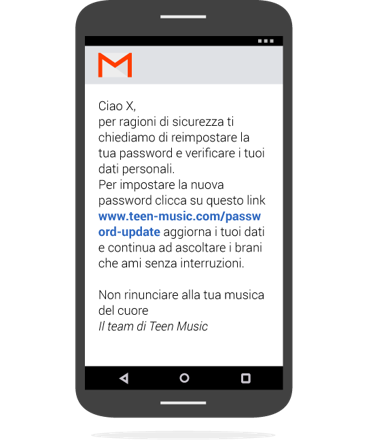
\includegraphics[scale=0.5]{Caso10.png}
\end{figure}
Il mittente è noreply@teen-music.it. Clicca su un link nel corpo della mail, ma si accorge che non finisce sulla solita pagina della piattaforma di musica, ma su una pagina che un po' le assomiglia e comunque ha il logo e i colori di quella di Teen Music. Gli viene chiesto di aggiornare i suoi dati e di reimpostare la password per motivi di sicurezza, chiedendogli però di inserire la password corrente unitamente al Codice Utente. La cosa lo insospettisce e si ferma.
\\\vspace{5mm}\\
\textbf{Cosa dovresti fare in una situazione simile?}
\begin{enumerate}
	\item Cliccare sul link per verificare se il messaggio è veritiero
	\item Chiudere il messaggio ed entrare nel proprio account e verificare la richiesta direttamente dalla piattaforma ufficiale del fornitore del servizio
	\item Verificare che la mail sia scritta in un italiano corretto
	\item Scrivere al servizio di supporto della piattaforma per verificare che stia inviando richieste di questa tipologia
	\item Aggiornare i dati personali e impostare nuovamente la pasword identica a quella precedente
	\item Inserire la password corrente e impostare la nuova password diversa da quella precedente
	\item Usare le impostazioni a disposizione per segnalare la mail come spam
\end{enumerate}
\vspace{5mm}
\textbf{Cosa avresti dovuto fare in caso fossi stato oggetto di truffa?}
\begin{enumerate}
	\item Parlare subito con i genitori o con un adulto di cui ti fidi
	\item Cambiare le password degli account online
	\item Cambiare computer e/o device mobile
	\item Avvisare tutti i propri contatti che potrebbero essere il prossimo bersaglio
	\item Nascondere l'accaduto ai propri contatti per non generare panico
	\item Suggerire ai propri contatti di cambiare preventivamente le loro password anche se non hanno aperto il link
\end{enumerate}
\subsection{Sconosciuti in rete}
A volte le persone fingono di essere qualcun altro online, in alcuni casi per fare degli scherzi, in altri allo scopo di rubare informazioni personali. Fortunatamente, ci sono degli elementi a cui prestare attenzione per verificare l' identità delle persone che ci contattano e identificare potenziali truffatori:
\begin{itemize}
	\item \textbf{L'immagine del profilo è reale?} Se l'immagine non è una foto di una persona reale ma un'immagine o illustrazione sii prudente, ma anche se la foto è di una persona reale, verifica se si vede bene o è sfocata. È facile nascondersi dietro a una foto sfocata. Inoltre non è difficile per i truffatori rubare foto di persone reali per creare profili falsi
	\item \textbf{Sul profilo ci sono informazioni dettagliate?} Se ci sono, sembrano scritte da una persona reale? Gli account falsi spesso non hanno molte informazioni nella sezione "Su di me" e quelle che ci sono potrebbero essere state inventate solo per creare un profilo falso e particolarmente accattivante
	\item \textbf{Da quanto tempo esiste questo account?} Sugli account falsi spesso non si trovano molti post, né molte interazioni sociali, questo significa che i contatti non conoscono bene il proprietario del profilo e non intergiscono con lui. I contatti o sono molto eterogenei tra loro per nazionalità e interessi o possono essere molto pochi se il profilo è stato appena aperto
\end{itemize}
\subsubsection{Caso di studio}
\label{sec:Caso11}
In chat ti scrive qualcuno che non conosci: "Ti ho visto nei corridoi di scuola oggi. 6 adorabile! Qual è il tuo indirizzo? Potrei venire da te x fare 2 chiacchiere."
\\\vspace{5mm}\\
\textbf{Cosa è più opportuno fare?}
\begin{enumerate}
	\item Ignorare il messaggio
	\item Bloccare questa persona
	\item Avviare comunque la conversazione con un "Chi sei?"
	\item "Vivo al numero 24 di via Roma, chi sei?"
\end{enumerate}
\subsubsection{Caso di studio}
\label{sec:Caso12}
Ricevi un messaggio da parte di qualcuno che non segui. "Ehi! Adoro i tuoi post, sei troppo divertente! Dammi il tuo numero di telefono, così possiamo parlare un pò e conoscerci meglio".
\\\vspace{5mm}\\
\textbf{Cosa consiglieresti di fare?}
\begin{enumerate}
	\item Di ignorare il messaggio
	\item Di rispondere "Ciao, ci conosciamo?"
	\item Di bloccare il contatto
	\item Di scrivergli "Grazie! Il mio numero è..."
\end{enumerate}

\begin{center}
	\begin{huge}
		\textbf{ATTENTO A CHI E A COME RISPONDI ONLINE!}
	\end{huge}
\end{center}

\pagebreak

\section{Custodisci le tue informazioni personali}
In questa sezione impararemo a come e cosa fare per proteggere i nostri segreti, attraverso la creazione di password efficaci e applicando strategie efficaci per custodiarle lontano da occhi indiscreti.
\subsection{Proteggi i tuoi segreti}
La tecnologia digitale facilita e consente di accedere a informazioni e servizi online, e di comunicare con amici, compagni, insegnanti in qualsiasi parte del mondo. Gli stessi strumenti potrebbero, però, permettere anche ad hacker e malintenzionati di rubare informazioni e usarle per danneggiare i nostri dispositivi, le nostre relazioni o la nostra reputazione. Proteggere tutto ciò che riguarda la nostra reputazione online significa adottare semplici ma importanti misure come usare il blocco schermo sui nostri dispositivi, fare attenzione alle informazioni personali che inseriamo che potrebbero andare perse o venire rubate e, soprattutto, scegliere delle ottime password.\\
Giusto quello si dice, ma tra mille mila siti, come ricordo tutto? Siamo sommersi da codici, parole chiave da ricordare per accedere a servizi di social network, email, musica o film in streaming, videogame, e per questo si tende ad utilizzare sempre la stessa. Basti pensare che nel 2017 la password più usata al mondo è stata «123456». Vediamo allora delle tecniche per, innanzittutto, creare delle password efficaci.
\begin{figure}[h!]
	\centering
	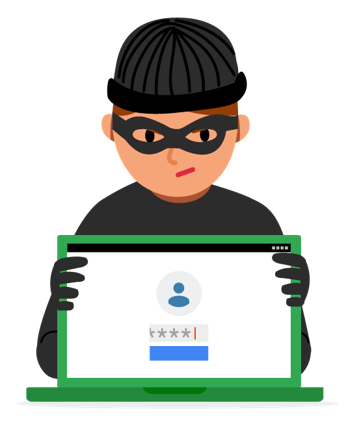
\includegraphics[scale=0.5]{Thieg.png}
\end{figure}
\subsection{Come creare una password efficace}
L'ingegneria sociale è una tecnica che consiste nello sfruttare siti come social network o applicativi di interazione online per parlare con la vittima e indurla a fornire informazioni su di sé, oppure per studiarne attentamente il profilo e carpire dettagli importanti che potrebbero rivelare una password (nomi di figli, fidanzati, amici, data di nascita o di matrimonio, etc.). Ma come fanno a rubarci le password?\\
Un attacco di forza bruta consiste nell’esecuzione di un programma capace di provare in brevissimo tempo moltissime combinazioni di password prese da un dizionario-database creato ad hoc, magari partendo da parole individuate grazie all'ingegneria sociale, per cercare di individuare quella giusta. In questo senso, tanto più le nostre password sono prive di collegamenti ad eventi che ci riguardano, tanto più sarà difficile individuarle.\\
\textbf{Ecco una lista di buone abitudini per la scelta della password:}
\begin{itemize}
	\item Scegliere una password lunga in quanto più sicura
	\item Rendere la password imprevedibile
	\item Non mettere dettagli personali al suo interno
	\item Usare una combinazione di lettere, numeri e caratteri speciali
\end{itemize}
Esempi di trucchi da usare sono quelli che andrò ad esplicare ora.\\
\begin{itemize}
	\item Gioca con gli acronimi di una frase semplice ma ben rappresentativa della tua identità; "Mi Chiamo Simona e Sono Nata il 3 Ottobre" potrebbe diventare \textit{\textbf{MCSeSNi3O}}	
	\item Costruisci una \textbf{passphrase}: crea un’unica stringa a partire da una frase composta e imprevedibile. Elimina gli spazi e, se credi, aggiungi le maiuscole all’inizio di ogni parola: "3 è il numero imperfetto" diventa \textit{\textbf{.3èilNumeroImperfetto}}
	\item Prendi la tua solita password e aggiungi caratteri extra alla fine (si chiama padding): "ioReetuRegina" può diventare \textit{\textbf{10ReetuRegina.11}} oppure \textit{\textbf{IoReetuRegina((11))}} oppure ancora \textit{\textbf{Io,Re,e,Tu,Regina,11}}
\end{itemize}
\subsubsection{Esercizio}
Quale tra le seguenti password sono efficaci?\\
\vspace{5mm}
\begin{center}
	\begin{tabular}{c|c}
		buongiornoprincipessa & Princi10Pessa.Mia \\ \hline
		IlikeScar\_fac3 & Sc4rf4c3 \\ \hline
		YMCA & SFIDT3 \\ \hline
		Siam03PiccoliPorcospin-) & SonoPazzoDit3
	\end{tabular}
\end{center}
\subsection{Verifica in due passaggi}
La verifica in due passaggi, o autenticazione a più fattori, è una misura di sicurezza che richiede due passaggi per effettuare l'accesso a un servizio. 
Solitamente si tratta di un ulteriore codice di verifica (oltre alla password) che si genera di volta in volta tramite applicativi, dispositivi o può arrivare anche via sms sul telefono. Esempi di dispositivi a due passaggi sono il codice monouso e il token USB.
\begin{figure}[h!]
	\centering
	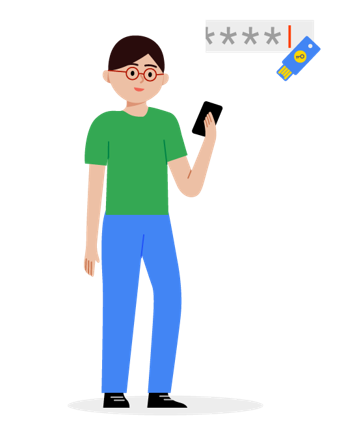
\includegraphics[scale=0.5]{Passaggi1.png}
\end{figure}
\subsubsection{Individua i fattori per la verifica a due passaggi}
\label{sec:Caso13}
\begin{itemize}
	\item Codice monouso via sms
	\item Inserire due volte la propria password
	\item USB token
	\item Codice monouso tramite APP
	\item Effettuare l'accesso due volte consecutivamente
	\item Effettuare l'accesso sempre dallo stesso dispositivo
	\item Codici monouso senza scadenza da stampare
\end{itemize}
\begin{figure}[h!]
	\centering
	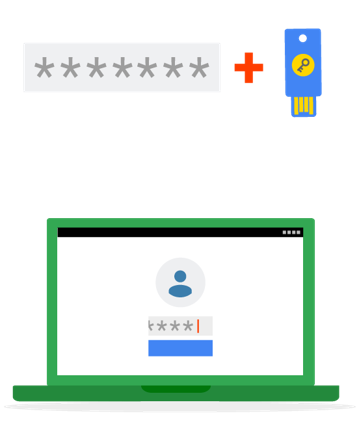
\includegraphics[scale=0.5]{Passaggi2.png}
\end{figure}
\subsubsection{Inndica se le seguenti frasi sono giuste o sbagliate}
\label{sec:Caso14}
\begin{itemize}
	\item Nelle password è meglio non usare la nostra data di nascita, ma quella di altri membri della nostra famiglia sì		
	\item Una password veramente sicura dovrebbe essere imprevedibile e contenere lettere, numeri e caratteri speciali		
	\item Una password con la nostra canzone o citazione preferita è certamente sicura
	\item Non è necessario utilizzare la verifica in due passaggi quando si tratta di profili social ma solo per account di posta elettronica o banking online		
	\item Una password non va condivisa con nessuno e per nessun motivo al mondo, neanche con un genitore
\end{itemize}
\subsection{Custodisci le tue password}
Ecco dei suggerimenti per cercare di non farti trafugare facilmente le password personali:
\begin{enumerate}
	\item Non utilizzare password già usate in passato e comuni ad altri nostri account
	\item Evitiamo di lasciare note con le password sul computer o sulla scrivania ed effettuiamo il log out specialmente quando accediamo ai nostri account da un pc pubblico o utilizzando una rete pubblica
	\item Se possibile, utilizziamo sempre le opzioni per il recupero dell'account
	\item Non diamo mai la nostra password a nessuno, tranne forse i genitori
\end{enumerate}
\textcolor{red}{Ricorda!} Il diritto alla privacy ed alla segretezza delle comunicazioni del minore si scontra con il diritto/dovere di vigilanza dei genitori. Infatti, non solo nel 99.9\% dei casi i contratti con i provider di rete sono intestati ai genitori anche se fruiti dai figli, ma il genitore ha il dovere di proteggere il ragazzo da eventuali pericoli ed è responsabile per quest’ultimo nel caso di azioni illecite.
\subsubsection{Caso di studio}
\label{sec:Caso15}
Pietro sta facendo un lavoro di gruppo a scuola. L’insegnante chiede di creare un nuovo account di posta elettronica che sarà usato dal gruppo. Pietro ha l’incarico di scegliere il nome dell’account e la password. Per ricordarla facilmente, sceglie quella che utilizza per i suoi account personali; per differenziarla aggiunge l’anno corrente e la condivide con i suoi compagni di gruppo. Qualche giorno dopo Pietro nota che la sua immagine su uno dei profili social è cambiata, ma non ricorda di essere stato lui a farlo. Prova ad accedervi senza riuscirci. Qualcuno ha eseguito l’accesso e cambiato la password. Si preoccupa perché quella è anche la password di altri account tra cui quello di posta elettronica.
\\\vspace{5mm}\\
\textbf{Cosa dovrebbe fare a questo punto Pietro?}
\begin{itemize}
	\item Creare un nuovo account e rinunciare subito ad accedere al vecchio		
	\item Abilitare sui siti su cui ha un account la verifica in due passaggi, laddove possibile
	\item Verificare sulla pagina di assistenza del provider di posta l’esistenza di un metodo di recupero password alternativo per il servizio di posta elettronica
	\item Cancellare o chiudere i suoi account con password simili a quella hackerata
	\item Cambiare radicalmente le password simili a quella hackerata usate per accedere ad altri account
\end{itemize}
\subsubsection{Caso di studio}
\label{sec:Caso16}
Sonia e Giorgia sono sempre state molto amiche, e come prova di fiducia si scambiano una password di accesso ad un account social. Quando Sonia inizia a mostrare interesse per un compagno di scuola e a passare meno tempo con Giorgia, questa, gelosa, entra sulla piattaforma usando le credenziali di Sonia e comincia a scrivere a suo nome post imbarazzanti e a inviare una serie di contenuti offensivi tramite messaggi privati ad alcuni contatti dell’amica.
\\\vspace{5mm}\\
\textbf{Cosa dovrebbe fare Sonia in una situazione del genere?}
\begin{itemize}
	\item Attivare la notifica di accesso da dispositivi diversi dal suo tramite sms
	\item Cambiare immediatamente password e altre password simili usate per altri account
	\item Inviare un messaggio ai destinatari dei messaggi spiegando l’accaduto
	\item Cancellare il suo account
	\item Sostituire la password con un’altra semplice per assicurarsi sempre l’accesso senza difficoltà
	\item Parlarne direttamente con Giorgia e/o con un adulto
\end{itemize}
\begin{center}
	\begin{huge}
		\textbf{CREA PASSWORD EFFICACI E TIENILE SEMPRE AL SICURO}
	\end{huge}
\end{center}
\pagebreak
\section{Diffondi la gentilezza}
In questa sezione impareremo a capire cos'è il cyberbullismo, a capire qual è il compito di ognuno di noi come educatore e a educare ed educarci alla gentilezza.
\subsection{Cyberbullismo}
La comunicazione online annulla quasi completamente il contatto reale, riduce l’empatia tra gli individui coinvolti, assottiglia le sfumature e, in alcuni casi, può dare adito a interpretazioni diverse rispetto a quanto accadrebbe nella vita reale, in una discussione di persona o al telefono. Anche i tempi, online, sono molto più serrati. Per questo, quando interagiamo online è importante ricordare che dietro ad ogni nome utente o avatar, quasi sempre c'è una persona in carne ed ossa, che prova sentimenti reali e merita di essere trattata con rispetto, e che potrebbe essere ferita da un messaggio, una battuta o un commento frettoloso o superficiale, anche se prodotto senza reale cattiveria.\\
Ma allora cos'è il \textbf{Cyberbullismo}? “Qualsiasi forma di pressione, aggressione, molestia, ricatto, ingiuria, denigrazione, diffamazione, furto d’identità, alterazione, acquisizione illecita, manipolazione, trattamento illecito di dati personali in danno di minorenni, realizzata per via telematica”.\\
\begin{figure}[h!]
	\centering
	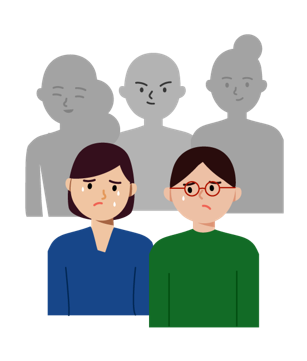
\includegraphics[scale=0.5]{Bullismo1.png}
\end{figure}
I soggetti coinvolti nel cyberbullismo sono sempre 3:
\begin{enumerate}
	\item Uno o più bulli
	\item Il bersaglio o vittima
	\item Persone terze che chiameremo testimoni o spettatori
\end{enumerate}
Il cyberbullismo si poggia sulla depersonalizzazione e sulla deresponsabilizzazione possibili in rete, poiché comunicando in maniera testuale non si partecipa direttamente allo stato emozionale delle persone che una comunicazione comporta.\\
Piccoli gesti di gentilezza possono fare una grande differenza online. Ma è vero anche il contrario: piccoli gesti spiacevoli online possono trasformarsi in qualcosa di molto brutto e dalle conseguenze tragiche. Ad esempio, un contenuto offensivo, allusivo, messo in rete da un bullo può essere condiviso a cascata dai testimoni, amplificando in maniera esponenziale l’effetto dell’aggressione, con risultati devastanti per la vittima che, anche a casa sua, non si sentirà mai sicura. Perché Internet è un luogo senza confini, pervasivo, capace di raggiungerlo ovunque.
\subsection{Tipologie di Cyberbullismo}
Il \textbf{Flaming} (da flame, fiamma) consiste nell’invio di messaggi offensivi allo scopo di innescare battaglie verbali online (ad esempio su una piattaforma di giochi online).\\
L’\textbf{Harassment} (molestia) è un comportamento simile al Flaming, ma si verifica quando vi è l'invio ripetuto di messaggi denigratori che ha come obiettivo ultimo quello di ferire qualcuno.\\
Quando si parla di \textbf{Cyberstalking} (persecuzione telematica), l’artefice dell’aggressione non si limita più a offese, ma perseguita la sua vittima con vere e proprie minacce, tanto da farle temere per la propria sicurezza fisica.\\
La \textbf{Denigrazione} avviene attraverso la diffusione di pettegolezzi o immagini imbarazzanti sulla vittima allo scopo di ridicolizzarla e danneggiarne la reputazione.\\
La \textbf{Sostituzione dell’identità} ha luogo quando il cyberbullo riesce ad accedere all’account della vittima e fingersi questa persona, inviando messaggi ai suoi contatti e a nome suo, allo scopo di rovinarne la reputazione.\\
Si parla di \textbf{Trickery} (raggiro) quando il cyberbullo rivela informazioni personali e riservate della vittima ottenute con l’inganno, ad esempio condividendo registrazioni di confidenze o chat o minacciando di farlo qualora questa non accetti di esaudire le sue richieste.\\
Cyberbullismo è anche \textbf{Escludere} la vittima da liste di gruppi online o piattaforme di gioco interattive. Infatti, oggi la leadership di un adolescente è dettata anche dai suoi amici online, non solo da quelli reali, e l’esclusione rappresenta una vera e propria punizione mirata a ledere la popolarità della vittima.\\
Il \textbf{Cyberbashing} o \textbf{Happy Slapping} (letteralmente “schiaffeggio allegro”) è la forma più estrema di cyberbullismo che consiste nella ripresa di atti di violenza nei confronti della vittima e la successiva condivisione del video sulle piattaforme social. Si tratta di un vero e proprio comportamento criminale.\\
\subsubsection{Di cosa si tratta?}
\begin{itemize}
	\item Insulti inviati ripetutamente in una chat di gruppo ad una persona sono da considerarsi uno scherzo?		
	\item Due ragazzi chiudono una compagna di classe in bagno, la convincono a spogliarsi e la riprendono. Non la sfiorano, ma diffondono il video online. In questo caso, oltre che di cyberbullismo, siamo in presenza di un reato?		
	\item Due amici carissimi si prendono spesso in giro e si scambiano le medesime battute anche online, utilizzando attributi spesso poco gentili. Questo atteggiamento è ascrivibile a cyberbullismo e reato?		
	\item Uno studente in anonimato invia un messaggio privato al professore intimandogli di alzare la media a tutta la classe, altrimenti la pagherà cara. È cyberbullismo?
\end{itemize}
\subsection{Combattere il Cyberbullismo}
Ecco delle semplici azioni che puoi applicare tutti i giorni per combattere tale fenomeno. Ricorda, non costano niente.
\begin{enumerate}
	\item Offrire il buon esempio: Rappresentare una voce equilibrata per il bullo e dimostrare gentilezza nei confronti della vittima aiuta a diffondere positività
	\item Essere amichevole: Comportarsi amichevolmente con la vittima, sia online che offline, può davvero fare la differenza. Questo dimostrerà che non sono soli e li aiuterà sia nel caso fossero vittime di bullismo sia nel caso si sentissero semplicemente tristi o incapaci di affrontare una situazione difficile
	\item Non incoraggiare comportamenti negativi assumendo il ruolo di “pubblico”: Non è bene mettere "mi piace", partecipare e rispondere a commenti o post offensivi. A volte i bulli si comportano aggressivamente per attirare l'attenzione; non vanno incoraggiati, ma ignorati
	\item Non far girare messaggi offensivi: Segnalare a chi ha mandato il messaggio che lo si trova sgradevole è un comportamento giusto e coraggioso, così come scrivere alla vittima per offrirle supporto. Significa prendere una posizione
	\item Segnalare i comportamenti persecutori: attraverso gli appositi strumenti di segnalazione online o parlandone con genitori, insegnanti, amici, fratelli o sorelle maggiori
\end{enumerate}
\subsubsection{Caso di studio}
\label{sec:Caso17}
Sandra è al primo anno delle superiori, e la sua migliore amica delle medie, Carmen, è capitata in un’altra classe. Sandra si trova bene con le sue nuove compagne di classe. Una di loro la invita ad una festa a casa sua, ma Carmen, gelosa, le dice di non andarci. Sandra trova ingiusta questa richiesta e decide di partecipare comunque alla festa. Qualche giorno dopo le fanno notare che esiste una pagina su un social network chiamata “Sandra, la regina delle sfigate”, piena di messaggi e confidenze che Sandra aveva condiviso privatamente con Carmen, oltre che foto imbarazzanti e private che la mettono a disagio di fronte ai coetanei. La pagina raccoglie sempre più fan e i commenti pesanti e offensivi nei suoi confronti si moltiplicano.
\\\vspace{5mm}\\
\textbf{Come potresti intervenire appena al corrente dell'accaduto?}
\begin{itemize}
	\item Segnalare la pagina creata
	\item Parlare a scuola dei comportamenti da bulli e delle conseguenze che possono derivarne, magari assistendo a documentari o chiedendo l'intervento di un esperto
	\item Coinvolgendo la famiglia di Sandra
	\item Punendo chi ha creato la pagina
	\item Invitando le migliori amiche di Sandra ad appoggiarla e sostenerla
	\item Dicendo a Sandra che non deve predersela, poiché si tratta di una ragazzata, ne uscirà più forte
\end{itemize}
\subsubsection{Esercizio}
\label{sec:Caso18}
Cosa consiglieresti di fare a una vittima di bullismo o a un testimone che abbia assistito a comportamenti scorretti online?
\begin{itemize}
	\item Di ripagare il cyber-bullo con la sua stessa moneta
	\item Di bloccare chi lo sta importunando
	\item Di segnalare o raccontare l'episodio a genitori, insegnanti, fratelli, sorelle o amici
	\item Di evitare di rispondere e lasciar correre. Passerà	
	\item Se necessario, di denunciare il caso alle forze dell’ordine
	\item Di rispondere con gentilezza	
	\item Di evitare di rispondere e parlarne con qualcuno di fiducia
	\item Di rispondere con minacce
	\item Di cambiare le impostazioni di privacy
\end{itemize}
\subsubsection{Esercizio sulla gentilezza}
\label{sec:Caso19}
Si può reagire alle emozioni negative in modo costruttivo, riformulando i commenti ostili e facendo più attenzione al tono che si utilizza durante la comunicazione online. Reagire positivamente a uno stimolo negativo può rendere la conversazione più interessante e più divertente ed è molto meglio che trovarsi a cercare di aggiustare una situazione complicata generata da un commento spiacevole. 
\\\vspace{5mm}\\
\textbf{Quali di questi commenti apparentemente banali andrebbero evitati?}
\begin{itemize}
	\item Lol, Stefano, sei l'unico della classe a non venire in gita. Sei proprio un poveraccio, costa troppo per te
	\item Mi spiace un sacco che Stefano non possa venire. Sarà per la prossima volta!
	\item Senza offesa, ma staresti meglio nella squadra dei principianti
	\item Sei più bella nelle foto quando hai un'espressione malinconica
	\item E' tremenda, ma chi le ha fatto credere di sapre cantare?
	\item Con quei denti che si ritrova non dovrebbe ridere in foto
	\item Ma nessuno le ha detto che ha una portaerei al posto del sedere?
	\item I genitori di Stefano sembrano due giovincelli, davvero simpatici!
\end{itemize}

\pagebreak

\section{Nel dubbio, parlane!}
Un errore, spesso commesso dagli adulti, è considerare Internet e tutti i suoi ambiti, siti, chat, app, messaggistica istantanea, un “mondo altro” rispetto a quello in cui trascorriamo la nostra giornata.\\
Spesso i ragazzi mostrano difficoltà a schierarsi dalla parte della vittima per “paura di fare la stessa fine”, ma in ogni classe ci sono soggetti più sensibili di altri: “Ammettiamolo! Lo sapevamo tutti che stava male”.\\
Truffe, frodi online, phishing, perdita di dati, violazione della propria privacy, sono fenomeni che quotidianamente coinvolgono tanto gli adulti quanto i ragazzi più giovani.\\
Molte volte è la scarsa consapevolezza del mezzo a generare questa tipologia di inconvenienti. I ragazzi spesso sentono gli adulti lontani e incapaci di poter comprendere i loro disagi o le situazioni che stanno vivendo.\\
\begin{center}
	\begin{large}
		\textbf{\textit{“Posso confidarmi con quella persona perché ci è passata e non mi giudicherà”.
		}}
	\end{large}
\end{center}
Gli adulti non sono dei giudici infallibili, anzi sono spesso essi stessi vittime dei tranelli (piccoli e grandi) presenti in rete, ma hanno l’esperienza e i mezzi per risolvere più efficacemente e velocemente i problemi e le situazioni spiacevoli e di imbarazzo che possono generarsi in rete
\begin{figure}[h!]
	\centering
	
\includegraphics[scale=0.5]{adults1.png}
\end{figure}
I testimoni, molte volte, pur non condividendone il comportamento, temono di diventare a loro volta vittime del bullo. Non comprendono la gravità dell’atto a cui stanno assistendo, e lo considerano uno scherzo, sottovalutando le conseguenze. Oppure provano piacere nell’assistere all’atto e partecipano all’episodio in forma indiretta, ad esempio filmando l’episodio o condividendolo sui social.
\subsubsection{Esercizio}
\label{sec:Caso20}
\textbf{Quali di questi suggerimenti ti sembrano validi per spingere i testimoni a raccontare eventuali episodi di cyberbullismo?}
\begin{itemize}
	\item Aprire una casella mail o dare un numero whatsapp a cui gli studenti possano scrivere per denunciare eventuali episodi.		
	\item Individuare i testimoni e parlare direttamente, biasimando la loro incapacità di denunciare e schierarsi dalla parte della vittima.		
	\item Avviare un discorso, che duri nel tempo, aperto a tutta la classe e che spinga i testimoni a riflettere sul loro ruolo.		
	\item Mettere a disposizione dei ragazzi un Box a scuola dove, anche in anonimato, possano descrivere e denunciare atti di bullismo o cyberbullismo nei confronti di qualsiasi studente.		
	\item Dichiarare in classe che chi tace o ha taciuto è complice del bullo.
\end{itemize}
\vspace{20mm}
\begin{figure}[h!]
	\centering
	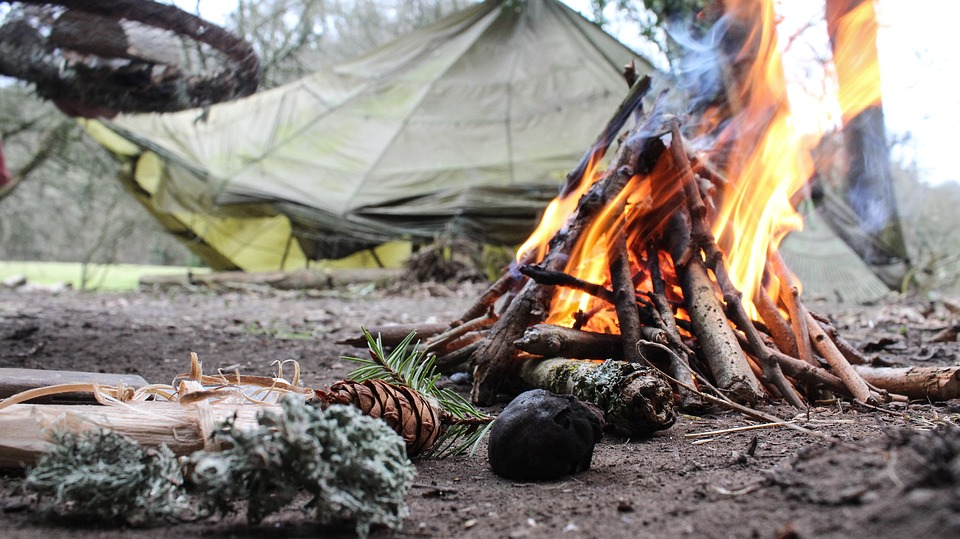
\includegraphics[scale=1.7]{Fuoco1.jpg}
\end{figure}

	\pagebreak
	
	\section{Soluzioni ai casi di studio}
	\subsection{Caso di studio \ref{sec:Caso1}}
		\begin{itemize}
			\item \textcolor{green}{Che sono ragazzi superficiali}
			\item \textcolor{red}{Che sono ragazzi divertenti e simpatici}
			\item \textcolor{green}{Che sono ragazzi poco attenti alla reputazione dei loro amici}
			\item \textcolor{red}{Che sono ragazzi abili con le nuove tecnologie}
		\end{itemize}
	\subsection{Caso di studio \ref{sec:Caso2}}
		\begin{itemize}
			\item \textcolor{red}{Quella di un ragazzo con una passione sana per l’arte, socievole e con uno spiccato senso civico}
			\item \textcolor{green}{Quella di un writer non autorizzato e privo di senso civico}
			\item \textcolor{green}{Quella di un ragazzo poco affidabile e senza alcun controllo da parte della famiglia: un giovane di quell’età che passa le nottate fuori di casa}
		\end{itemize}
	\subsection{Caso di studio \ref{sec:Caso3}}
	\begin{itemize}
		\item \textcolor{green}{Di inviare la foto in un messaggio privato}
		\item \textcolor{red}{Di impostare "Solo amici" sul suo profilo}
		\item \textcolor{red}{Di impostare "Tutti" sul profilo della sua amica}
		\item \textcolor{green}{Di esplicitare, dopo qualche giorno, che si trattava di uno scherzo e/o eliminare l'immagine}
	\end{itemize}
\subsection{Caso di studio \ref{sec:Caso4}}
\begin{itemize}
	\item \textcolor{green}{Di controllare le impostazioni e le notifiche sui tag}
	\item \textcolor{red}{Di evitare di farsi riprendere}
	\item \textcolor{red}{Di impostare il video come "non visibile sul suo profilo"}
	\item \textcolor{green}{Di segnalare il video}
\end{itemize}
\subsection{Cado di studio \ref{sec:Caso5}}
\begin{itemize}
	\item \textcolor{green}{Non condividere mai e per nessuna ragione una password (per intero) in una chat}
	\item \textcolor{red}{Cancellare il gruppo dopo la festa}
	\item \textcolor{red}{Cancellare il messaggio dopo la festa}
	\item \textcolor{red}{Scrivere la password in più messaggi differenti}
\end{itemize}
\subsection{Caso di studio \ref{sec:Caso6}}
\begin{itemize}
	\item \textcolor{green}{Aspettare il padre}		
	\item \textcolor{green}{Chiedere al padre di condividere i dati della carta di credito a pezzi e su piattaforme e canali differenti	}	
	\item \textcolor{red}{Fotografare la carta e inviare una foto invece dei dati}	
	\item \textcolor{red}{Condividere i dati della carta via mail}	
	\item \textcolor{red}{Condividerli tutti contemporaneamente su una chat}
\end{itemize}
\subsection{Caso di studio \ref{sec:Caso7}}
\begin{itemize}
	\item \textcolor{green}{Ignorare il messaggio e non cliccare}
	\item \textcolor{red}{Cliccare per capire di cosa si tratta}
	\item \textcolor{red}{Inviarlo a quante più amiche possibili}		
	\item \textcolor{green}{Diffidare in futuro di questo tipo di messaggi e cancellarlo senza cliccare sul link}	
	\item \textcolor{green}{Informare tutta la classe delle truffe che si nascondono dietro questo tipo di messaggi}
\end{itemize}
\subsection{Caso di studio \ref{sec:Caso8}}
\begin{enumerate}
	\item \textcolor{red}{1db3w0assistenza@teen-music.com}		
	\item \textcolor{red}{http://online.da.teenmusic.da-it.upadate.com}
	\item \textcolor{green}{https://titolari.teenmusic.it/portal/server.pt}	
	\item \textcolor{red}{http://kolemsveta.cz/www.teenmusic.it/index.php}	
	\item \textcolor{red}{http://login.teenmusic.access.it}		
	\item  \textcolor{red}{assistenza@teenmusic.ru}		
	\item \textcolor{red}{https://80.574.215.39.teenmusic-italia.it}
	\item \textcolor{green}{noreply@teenmusic.it}		
	\item \textcolor{red}{www.teenmusic.com.personal.login}
\end{enumerate}
\subsection{Caso di studio \ref{sec:Caso9}}
\begin{enumerate}
	\item \textcolor{green}{Controllare l'indirizzo email del mittente}	
	\item \textcolor{green}{Controllare se l’allegato ha un'estensione immediatamente eseguibile (es. .exe, .bat o ancora .msi)}	
	\item \textcolor{green}{Contattare la polizia postale}
	\item \textcolor{red}{Spegnere il PC nella speranza che si resetti}	
	\item \textcolor{red}{Staccare la corrente elettrica e non accendere il PC per 7 giorni consecutivi}
	\item \textcolor{orange}{Scaricare un Antivirus}
\end{enumerate}
\subsection{Caso di studio \ref{sec:Caso10}}
\begin{enumerate}
	\item \textcolor{red}{Cliccare sul link per verificare se il messaggio è veritiero}
	\item \textcolor{green}{Chiudere il messaggio ed entrare nel proprio account e verificare la richiesta direttamente dalla piattaforma ufficiale del fornitore del servizio}
	\item \textcolor{green}{Verificare che la mail sia scritta in un italiano corretto}
	\item \textcolor{green}{Scrivere al servizio di supporto della piattaforma per verificare che stia inviando richieste di questa tipologia}
	\item \textcolor{red}{Aggiornare i dati personali e impostare nuovamente la pasword identica a quella precedente}
	\item \textcolor{red}{Inserire la password corrente e impostare la nuova password diversa da quella precedente}
	\item \textcolor{green}{Usare le impostazioni a disposizione per segnalare la mail come spam}
\end{enumerate}
\vspace{10mm}
\begin{enumerate}
	\item \textcolor{green}{Parlare subito con i genitori o con un adulto di cui ti fidi}
	\item \textcolor{green}{Cambiare le password degli account online}
	\item \textcolor{red}{Cambiare computer e/o device mobile}
	\item \textcolor{green}{Avvisare tutti i propri contatti che potrebbero essere il prossimo bersaglio}
	\item \textcolor{red}{Nascondere l'accaduto ai propri contatti per non generare panico}
	\item \textcolor{red}{Suggerire ai propri contatti di cambiare preventivamente le loro password anche se non hanno aperto il link}
\end{enumerate}
\subsection{Caso di studio \ref{sec:Caso11}}
\begin{enumerate}
	\item \textcolor{green}{Ignorare il messaggio}
	\item \textcolor{green}{Bloccare questa persona}
	\item \textcolor{red}{Avviare comunque la conversazione con un "Chi sei?"}
	\item \textcolor{red}{"Vivo al numero 24 di via Roma, chi sei?"}
\end{enumerate}
\subsection{Caso di studio \ref{sec:Caso12}}
\begin{enumerate}
	\item \textcolor{green}{Di ignorare il messaggio}
	\item \textcolor{green}{Di rispondere "Ciao, ci conosciamo?"}
	\item \textcolor{green}{Di bloccare il contatto}
	\item \textcolor{red}{Di scrivergli "Grazie! Il mio numero è..."}
\end{enumerate}
\subsection{Caso di studio \ref{sec:Caso13}}
\begin{itemize}
	\item \textcolor{green}{Codice monouso via sms}
	\item \textcolor{red}{Inserire due volte la propria password}
	\item \textcolor{green}{USB token}
	\item \textcolor{green}{Codice monouso tramite APP}
	\item \textcolor{red}{Effettuare l'accesso due volte consecutivamente}
	\item \textcolor{red}{Effettuare l'accesso sempre dallo stesso dispositivo}
	\item \textcolor{green}{Codici monouso senza scadenza da stampare}
\end{itemize}
\subsection{Caso di studio \ref{sec:Caso14}}
\begin{itemize}
	\item \textcolor{red}{Nelle password è meglio non usare la nostra data di nascita, ma quella di altri membri della nostra famiglia sì}	
	\item \textcolor{green}{Una password veramente sicura dovrebbe essere imprevedibile e contenere lettere, numeri e caratteri speciali}	
	\item \textcolor{red}{Una password con la nostra canzone o citazione preferita è certamente sicura}
	\item \textcolor{red}{Non è necessario utilizzare la verifica in due passaggi quando si tratta di profili social ma solo per account di posta elettronica o banking online}
	\item \textcolor{red}{Una password non va condivisa con nessuno e per nessun motivo al mondo, neanche con un genitore}
\end{itemize}
\subsection{Caso di studio \ref{sec:Caso15}}
\begin{itemize}
	\item \textcolor{red}{Creare un nuovo account e rinunciare subito ad accedere al vecchio}	
	\item \textcolor{green}{Abilitare sui siti su cui ha un account la verifica in due passaggi, laddove possibile}
	\item \textcolor{green}{Verificare sulla pagina di assistenza del provider di posta l’esistenza di un metodo di recupero password alternativo per il servizio di posta elettronica}
	\item \textcolor{red}{Cancellare o chiudere i suoi account con password simili a quella hackerata}
	\item \textcolor{green}{Cambiare radicalmente le password simili a quella hackerata usate per accedere ad altri account}
\end{itemize}
\subsection{Caso di studio \ref{sec:Caso16}}
\begin{itemize}
	\item \textcolor{green}{Attivare la notifica di accesso da dispositivi diversi dal suo tramite sms}
	\item \textcolor{green}{Cambiare immediatamente password e altre password simili usate per altri account}
	\item \textcolor{green}{Inviare un messaggio ai destinatari dei messaggi spiegando l’accaduto}
	\item \textcolor{red}{Cancellare il suo account}
	\item \textcolor{red}{Sostituire la password con un’altra semplice per assicurarsi sempre l’accesso senza difficoltàt}
	\item \textcolor{green}{Parlarne direttamente con Giorgia e/o con un adulto}
\end{itemize}
\subsection{Caso di studio \ref{sec:Caso17}}
\begin{itemize}
	\item \textcolor{green}{Segnalare la pagina creata}
	\item \textcolor{green}{Parlare a scuola dei comportamenti da bulli e delle conseguenze che possono derivarne, magari assistendo a documentari o chiedendo l'intervento di un esperto}
	\item \textcolor{green}{Coinvolgendo la famiglia di Sandra}
	\item \textcolor{red}{Punendo chi ha creato la pagina}
	\item \textcolor{green}{Invitando le migliori amiche di Sandra ad appoggiarla e sostenerla}
	\item \textcolor{red}{Dicendo a Sandra che non deve predersela, poiché si tratta di una ragazzata, ne uscirà più forte}
\end{itemize}
\subsection{Caso di studio \ref{sec:Caso18}}
\begin{itemize}
	\item \textcolor{red}{Di ripagare il cyber-bullo con la sua stessa moneta}
	\item \textcolor{green}{Di bloccare chi lo sta importunando}
	\item \textcolor{green}{Di segnalare o raccontare l'episodio a genitori, insegnanti, fratelli, sorelle o amici}
	\item \textcolor{red}{Di evitare di rispondere e lasciar correre. Passerà}	
	\item \textcolor{green}{Se necessario, di denunciare il caso alle forze dell’ordine}
	\item \textcolor{green}{Di rispondere con gentilezza}	
	\item \textcolor{green}{Di evitare di rispondere e parlarne con qualcuno di fiducia}
	\item \textcolor{red}{Di rispondere con minacce}
	\item \textcolor{green}{Di cambiare le impostazioni di privacy}
\end{itemize}
\subsection{Caso di studio \ref{sec:Caso19}}
\begin{itemize}
	\item \textcolor{red}{Lol, Stefano, sei l'unico della classe a non venire in gita. Sei proprio un poveraccio, costa troppo per te}
	\item \textcolor{green}{Mi spiace un sacco che Stefano non possa venire. Sarà per la prossima volta!}
	\item \textcolor{red}{Senza offesa, ma staresti meglio nella squadra dei principianti}
	\item \textcolor{green}{Sei più bella nelle foto quando hai un'espressione malinconica}
	\item \textcolor{red}{E' tremenda, ma chi le ha fatto credere di sapre cantare?}
	\item \textcolor{red}{Con quei denti che si ritrova non dovrebbe ridere in foto}
	\item \textcolor{red}{Ma nessuno le ha detto che ha una portaerei al posto del sedere?}
	\item \textcolor{green}{I genitori di Stefano sembrano due giovincelli, davvero simpatici!}
\end{itemize}
\subsection{Caso di studio \ref{sec:Caso20}}
\begin{itemize}
	\item \textcolor{green}{Aprire una casella mail o dare un numero whatsapp a cui gli studenti possano scrivere per denunciare eventuali episodi.}		
	\item \textcolor{red}{Individuare i testimoni e parlare direttamente, biasimando la loro incapacità di denunciare e schierarsi dalla parte della vittima.}		
	\item \textcolor{green}{Avviare un discorso, che duri nel tempo, aperto a tutta la classe e che spinga i testimoni a riflettere sul loro ruolo.}		
	\item \textcolor{green}{Mettere a disposizione dei ragazzi un Box a scuola dove, anche in anonimato, possano descrivere e denunciare atti di bullismo o cyberbullismo nei confronti di qualsiasi studente.}		
	\item \textcolor{red}{Dichiarare in classe che chi tace o ha taciuto è complice del bullo.}
\end{itemize}

\end{document}
